%%%%%%%%%%%%%%%%%%%%%%%%%%%%%%%%%%%%%%%%%
% Beamer Presentation
% LaTeX Template
% Version 2.0 (March 8, 2022)
%
% This template originates from:
% https://www.LaTeXTemplates.com
%
% Author:
% Vel (vel@latextemplates.com)
%
% License:
% CC BY-NC-SA 4.0 (https://creativecommons.org/licenses/by-nc-sa/4.0/)
%
%%%%%%%%%%%%%%%%%%%%%%%%%%%%%%%%%%%%%%%%%

%----------------------------------------------------------------------------------------
%	PACKAGES AND OTHER DOCUMENT CONFIGURATIONS
%----------------------------------------------------------------------------------------





\documentclass[
	10pt, % Set the default font size, options include: 8pt, 9pt, 10pt, 11pt, 12pt, 14pt, 17pt, 20pt
	%t, % Uncomment to vertically align all slide content to the top of the slide, rather than the default centered
	%aspectratio=169, % Uncomment to set the aspect ratio to a 16:9 ratio which matches the aspect ratio of 1080p and 4K screens and projectors
]{beamer}

\graphicspath{{figures/}{./}} % Specifies where to look for included images (trailing slash required)




\usepackage{booktabs} % Allows the use of \toprule, \midrule and \bottomrule for better rules in tables
\usepackage{multimedia}
\usepackage{hyperref}
\usepackage{outlines}
\usepackage{float}
% \usepackage{caption}
\usepackage{subcaption}
\usepackage{cases}



% Extra 
\usepackage{siunitx}


% \usepackage[backend=bibtex, 
%             style=phys, 
%             biblabel=brackets]{biblatex}



%----------------------------------------------------------------------------------------
%	THEME
%----------------------------------------------------------------------------------------

\usetheme{Madrid} %%%
\usefonttheme{default} % Typeset using the default sans serif font
% \usecolortheme{dolphin}
\definecolor{myblue}{RGB}{138,162,247}
\setbeamercolor{structure}{fg=myblue}
\setbeamercolor{section in head/foot}{bg=myblue}


%\usepackage{mathptmx} % Use the Times font for serif text
\usepackage{palatino} % Use the Palatino font for serif text

%\usepackage{helvet} % Use the Helvetica font for sans serif text
\usepackage[default]{opensans} % Use the Open Sans font for sans serif text
%\usepackage[default]{FiraSans} % Use the Fira Sans font for sans serif text
%\usepackage[default]{lato} % Use the Lato font for sans serif text

\useinnertheme{circles}
\useoutertheme{default}

% \setbeamertemplate{footline} % Uncomment this line to remove the footer line in all slides
% \setbeamertemplate{footline}[page number] % Uncomment this line to replace the footer line in all slides with a simple slide count
\setbeamertemplate{navigation symbols}{} % Uncomment this line to remove the navigation symbols from the bottom of all slides


% \usepackage{textpos} 
% \addtobeamertemplate{frametitle}{}{%
%     \begin{textblock*}{100mm}(0.96\textwidth,-0.85cm)
%         
\includegraphics[height=0.8cm,width=0.8cm]{UiO_segl_pos-eps-converted-to.pdf}
%     \end{textblock*}}


%----------------------------------------------------------------------------------------
%	PRESENTATION INFORMATION
%----------------------------------------------------------------------------------------

\title[Predicting Graphene Kirigami Friction]{Predicting Frictional Properties of Graphene Kirigami Using Molecular Dynamics and Neural Networks}
\subtitle{Designs for a negative friction coefficient} 
\author[Mikkel Metzsch Jensen]{Mikkel Metzsch Jensen}
\institute[UiO]{University of Oslo}
\date[Juni 02, 2023]{Juni 02, 2023}

\titlegraphic{\flushleft
\includegraphics[width=0.5\textwidth]{figures/MN_FYSISK_A_ENG.pdf}}

% \titlegraphic{\vspace{4cm}\flushright\includegraphics[width=2cm,height=2cm]{example-image-a}} 


\setbeamertemplate{bibliography item}{\insertbiblabel}
\usepackage[backend=bibtex, 
            style=phys, 
            biblabel=brackets]{biblatex}
\addbibresource{bibliography.bib}




%----------------------------------------------------------------------------------------
\begin{document}

%----------------------------------------------------------------------------------------
%	TITLE SLIDE
%----------------------------------------------------------------------------------------

\begin{frame}
	\titlepage % Output the title slide, automatically created using the text entered in the PRESENTATION INFORMATION block above
\end{frame}

%----------------------------------------------------------------------------------------
%	BODY
%----------------------------------------------------------------------------------------

\begin{frame}{Outline}
    \tableofcontents
\end{frame}


\section{Introduction} %%%%%%%%%%%%%%%%%%%%%%%%%%%%%%%%%%%%%%%%%%%%%%%%%%%%%%%%%%%%%
\subsection{Thesis overview}

\begin{frame}{Overview}
	\framesubtitle{Three main parts}
	
	\begin{enumerate}
		\setlength\itemsep{1em}
		\item \textbf{Sheet kirigami}: Alter a graphene sheet using atomic scale cuts and stretching
		\item \textbf{Forward simulation}: Calculate the frictional properties of the sheet using MD simulations
		\item \textbf{Accelerated search}: Use machine learning to replace the MD simulations and perform an accelerated search for new designs
	\end{enumerate}
	\vspace{2mm}
	
	Can we control the frictional properties of a graphene sheet using this technique?
	% \begin{itemize}
	% 	\item Can we utilize a coupling between load and stretch?
	% 	\item Negative friction coefficients
	% \end{itemize}
	
\end{frame}


\subsection{Motivation}


\begin{frame}
	\frametitle{Motivation}

	\begin{itemize}
		\item Kirigami: Variation of origami with cuts permitted
		\item Desgins: Macroscale $\to$ nanoscale
	\end{itemize}
	\vspace*{10px}

	\begin{figure}
		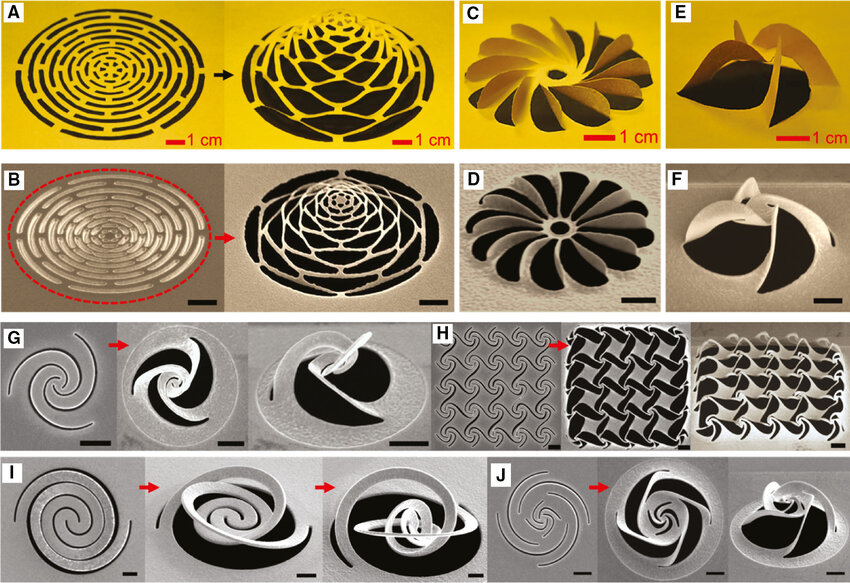
\includegraphics[height=0.55\textheight]{figures/kirigami_example.jpg}
		\caption{Example of macroscale Kirigami designs implemented on a nanoscale using a focused ion beam (FIB). Black scale bars: \SI{1}{\mu m}. Reproduced from~\cite{Li_2018}.}
	\end{figure}	
\end{frame}


\begin{frame}{Motivation}
	\framesubtitle{Out-of-plane buckling}
	\vspace{0.5cm}
	\begin{itemize}
		\item Hanakata et al. \cite{Hanakata_2018,Hanakata_2020} found out-of-plane buckling with Kirigami designs
		\item Surface properties is predicted to be important for friction properties
		\begin{itemize}
			\item Contact area
			\item Commensurability
		\end{itemize}
	\end{itemize}
	% \vspace{1cm}

	\begin{figure}[H]
		\centering
		\begin{subfigure}[b]{0.49\textwidth}
			\centering
			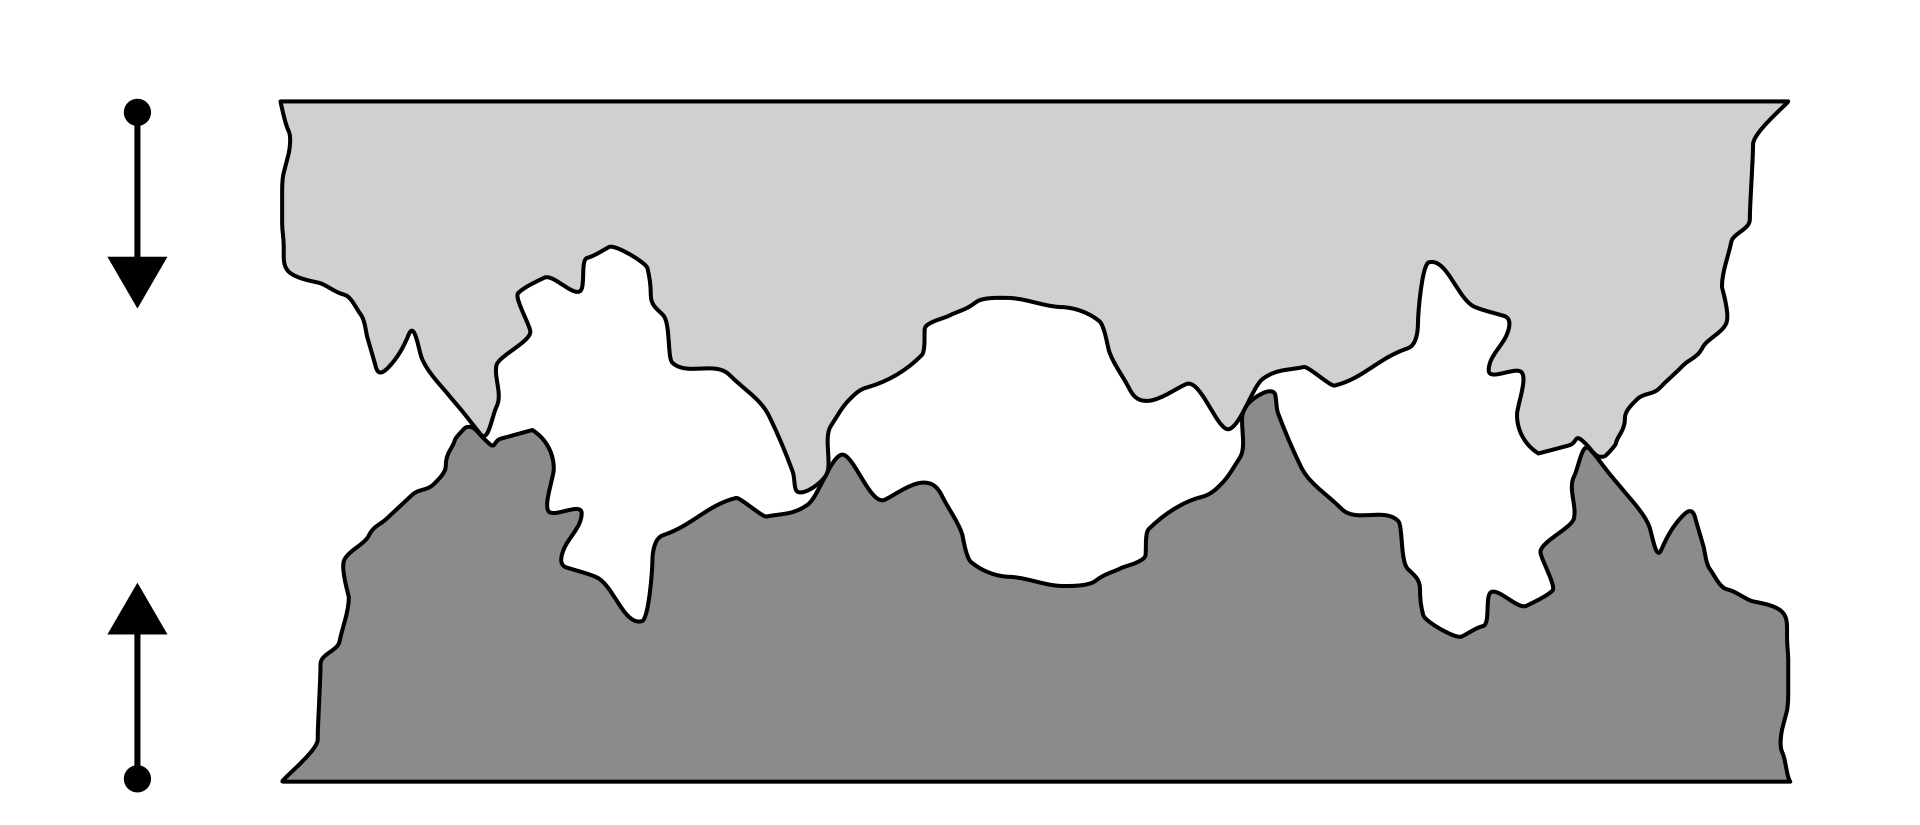
\includegraphics[width=\textwidth]{figures/asperities_top.png}
			\caption{Low load.}
			\label{fig:asp_left}
		\end{subfigure}
		\hfill
		\begin{subfigure}[b]{0.49\textwidth}
			\centering
			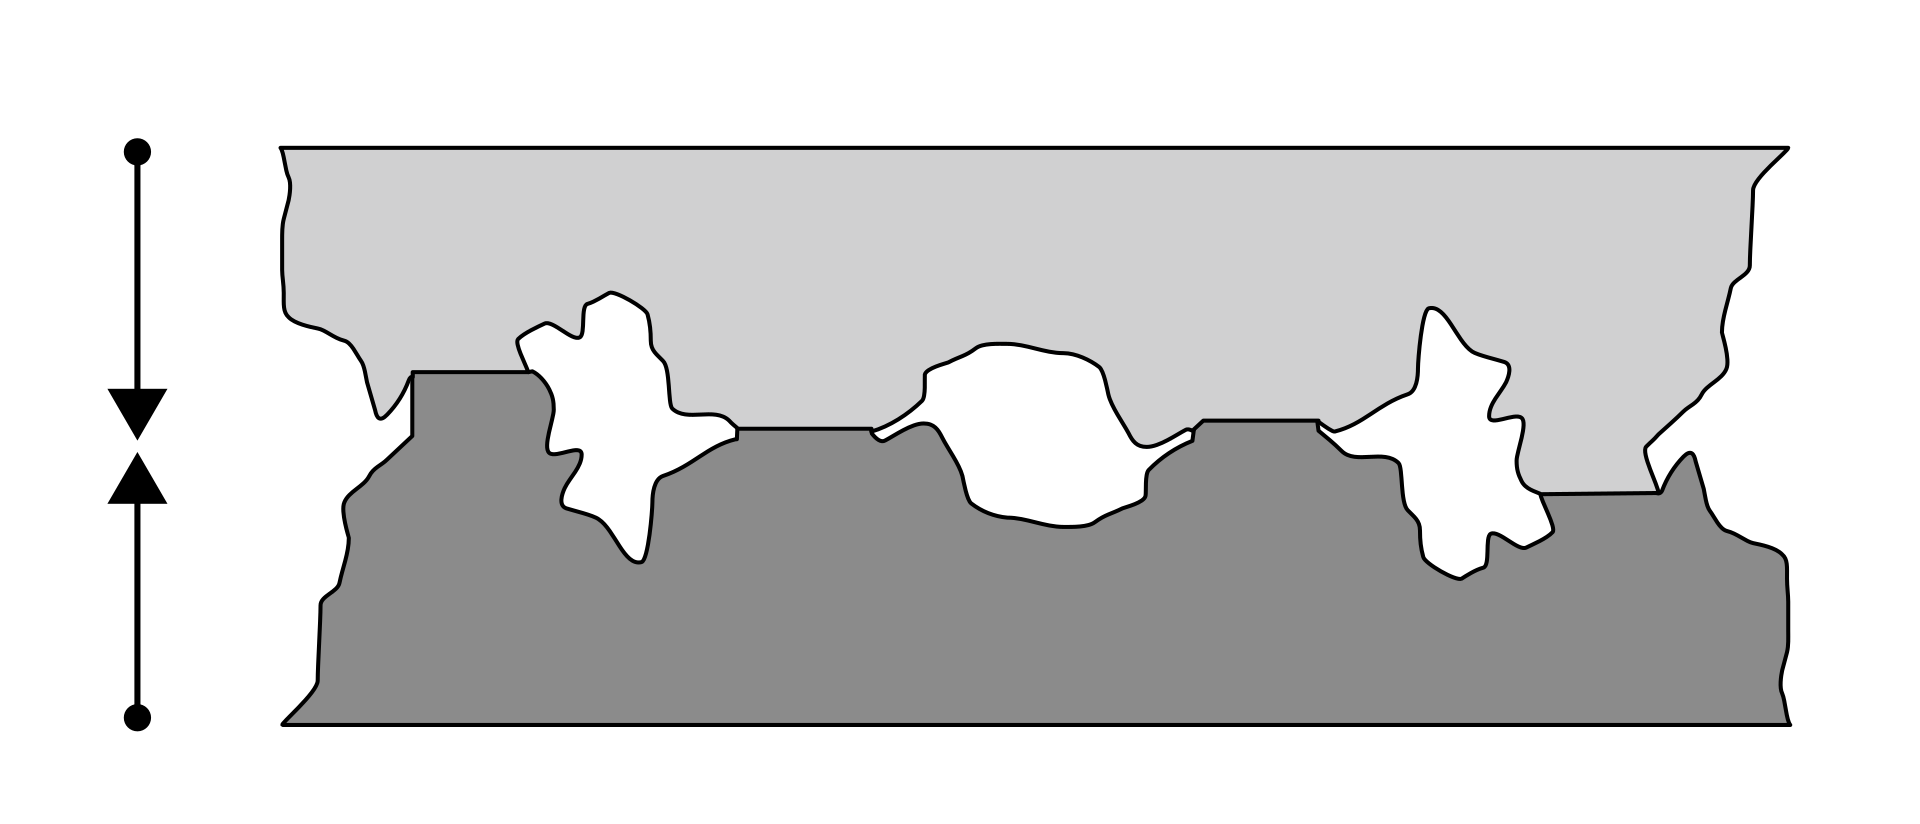
\includegraphics[width=\textwidth]{figures/asperities_bottom.png}
			\caption{High load.}
			\label{fig:asp_right}
		\end{subfigure}
		% \hfill
		\caption{Reproduced from~\cite{wiki:asperities}.}
	\end{figure}
	  

\end{frame}
	


\section{Creating a graphene Kirigami system} %%%%%%%%%%%%%%%%%%%%%%%%%%%%%%%%%%%%%%%%%%%%%%%%%%%%%%%%%%%%%
\subsection{System setup}
\subsection{Kirigami}




\section{Pilot study} %%%%%%%%%%%%%%%%%%%%%%%%%%%%%%%%%%%%%%%%%%%%%%%%%%%%%%%%%%%%%
\subsection{Friction metrics}
\subsection{Out-of-plane buckling}
\subsection{Friction-strain profiles}
\subsection{Negative friction coefficient}


\section{Kirigami configuration search} %%%%%%%%%%%%%%%%%%%%%%%%%%%%%%%%%%%%%%%%%%%%%%%%%%%%%%%%%%%%%
\subsection{Machine learning}
\subsection{Accelerated search}



\section{Summary and outlook} %%%%%%%%%%%%%%%%%%%%%%%%%%%%%%%%%%%%%%%%%%%%%%%%%%%%%%%%%%%%%



\begin{frame}%[allowframebreaks]
	\frametitle{References}
	\printbibliography
	% \bibliographystyle{apalike}
	% \bibliographystyle{plain}
	% \printbibliography
	% \bibliography{./presentation/bibliography.bib}
\end{frame}



\end{document} 


